% !TEX root = ../ApproxDA-TransUNet.tex
\section{Controlled Ablations}
\label{sec:understanding}

Each ablation varies one approximation parameter while all others, the backbone, and the training protocol are fixed.

\subsection{Window Size and Empirical Window Sensitivity}
\label{sec:window}

\begin{table}[t]
  \caption{DSC (\%) Versus Window Size $M$ (PAM-only Routing, $r{=}32$). Range $=\max_M \mathrm{DSC}(M) - \min_M \mathrm{DSC}(M)$.}
  \label{tab:window}
  \centering
  \footnotesize
  \setlength{\tabcolsep}{5pt}
  \begin{tabular}{@{}lccc@{}}
    \toprule
    Setting & Synapse & Kvasir-SEG & ISIC 2018 \\
    \midrule
    $M{=}7$                 & \tbd{78.64} & \tbd{89.53} & \tbd{89.41} \\
    $M{=}28$                & \tbd{\textbf{80.94}} & \tbd{89.54} & \tbd{\textbf{89.55}} \\
    $M{=}56$                & \tbd{78.90} & \tbd{\textbf{90.17}} & \tbd{89.05} \\
    $M{=}112$ (global, low-rank) & \tbd{79.44} & \tbd{89.56} & \tbd{89.51} \\
    \midrule
    Range                   & \tbd{2.30} & \tbd{0.64} & \tbd{0.50} \\
    \midrule
    DA-TransUNet (re-trained) & \tbd{--} & \tbd{88.44} & \tbd{88.43} \\
    \bottomrule
  \end{tabular}
\end{table}

\begin{figure}[t]
\centering
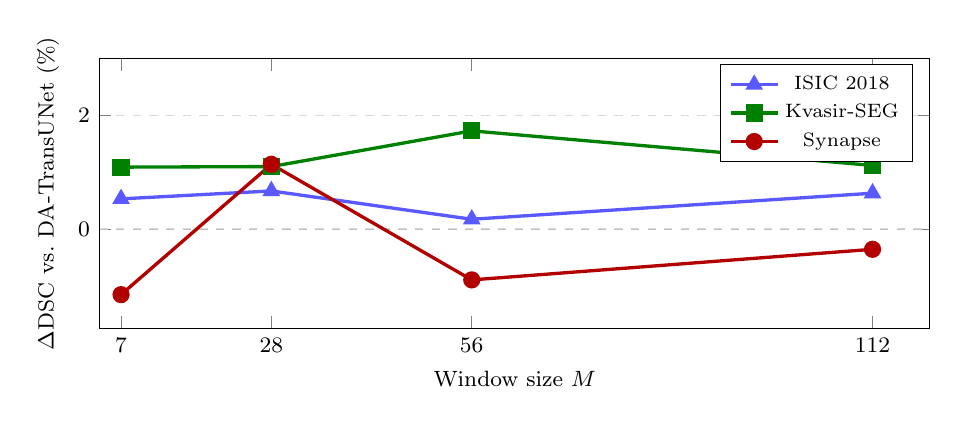
\begin{tikzpicture}
\begin{axis}[
  width=\columnwidth, height=5.0cm,
  xlabel={Window size $M$},
  ylabel={$\Delta$DSC vs.\ DA-TransUNet (\%)},
  ymin=-1.75, ymax=3.0,
  xtick={7,28,56,112},
  xmin=4, xmax=120,
  ymajorgrids=true,
  grid style={dashed,gray!30},
  tick label style={font=\footnotesize},
  label style={font=\footnotesize},
  legend style={font=\scriptsize, at={(0.98,0.98)}, anchor=north east},
  every axis plot/.append style={very thick, mark size=2.5pt},
]
\addplot[dashed, gray!50, very thin, forget plot] coordinates {(4,0)(120,0)};
\addplot[color=blue!65, mark=triangle*] coordinates {(7,0.53) (28,0.67) (56,0.17) (112,0.63)};
\addlegendentry{ISIC 2018}
\addplot[color=green!50!black, mark=square*] coordinates {(7,1.09) (28,1.10) (56,1.73) (112,1.12)};
\addlegendentry{Kvasir-SEG}
\addplot[color=red!70!black, mark=*] coordinates {(7,-1.16) (28,1.14) (56,-0.90) (112,-0.36)};
\addlegendentry{Synapse}
\end{axis}
\end{tikzpicture}
\caption{DSC difference to DA-TransUNet versus window size $M$ (PAM-only routing, $r{=}32$); raw values in Table~\ref{tab:window}. \tbd{Curves from the BIBM runs; to be regenerated from the re-trained models.}}
\label{fig:dsc_vs_m}
\end{figure}
% TODO(figure): recompute coordinates as DSC(M) - DSC(re-trained DA-TransUNet)
% from Table tab:window after the re-runs.

Table~\ref{tab:window} and Fig.~\ref{fig:dsc_vs_m} vary only $M$. On Synapse, DSC peaks at an intermediate window ($M{=}28$) and drops for both smaller and larger windows, giving a \tbd{2.30}-point range. Kvasir-SEG and ISIC 2018 are \tbd{3.6--4.6}$\times$ less sensitive, with ranges of \tbd{0.64} and \tbd{0.50} points. We summarize this behavior by the \emph{empirical window sensitivity}
\[
  S_{\mathrm{window}} = \max_M \mathrm{DSC}(M) - \min_M \mathrm{DSC}(M),
\]
which describes how this architecture responds to $M$ on a given dataset; it is not an independent predictor of a task's contextual requirement, and three datasets are not sufficient to establish it as a task property. The observed difference is consistent with multi-organ CT segmentation depending more on inter-organ spatial context than polyp and skin-lesion segmentation, which are largely determined by local appearance and boundary contrast.

The sensitivity also bounds how much the choice of $M$ matters in practice: on Kvasir-SEG and ISIC 2018 any tested window stays within \tbd{0.64} points of the best, whereas on Synapse the window must be tuned. On all three datasets the best window \tbd{exceeds} the re-trained DA-TransUNet, suggesting a locality-induced bias. This comparison changes both the attention approximation and the routing (PAM-only instead of PAM + CAM); the exact-attention rows of Table~\ref{tab:factors} isolate the approximation itself. Note that $M{=}112$ keeps the rank-32 projection and therefore differs from full PAM.

Fig.~\ref{fig:attn_map} visualizes the effect of the window on Kvasir-SEG. On 10 test images, windowed PAM ($M{=}7$) places $62.3\%$ of its contribution inside the polyp region, compared with $34.2\%$ for global PAM ($M{=}112$), and the windowed share is higher in 9 of the 10 images. Windowed attention concentrates on polyp boundaries, whereas global attention spreads over surrounding tissue. This observation is consistent with the locality interpretation but does not by itself establish a causal link to accuracy. \tbd{Maps from the BIBM checkpoints; to be regenerated.}

\begin{figure}[t]
  \centering
  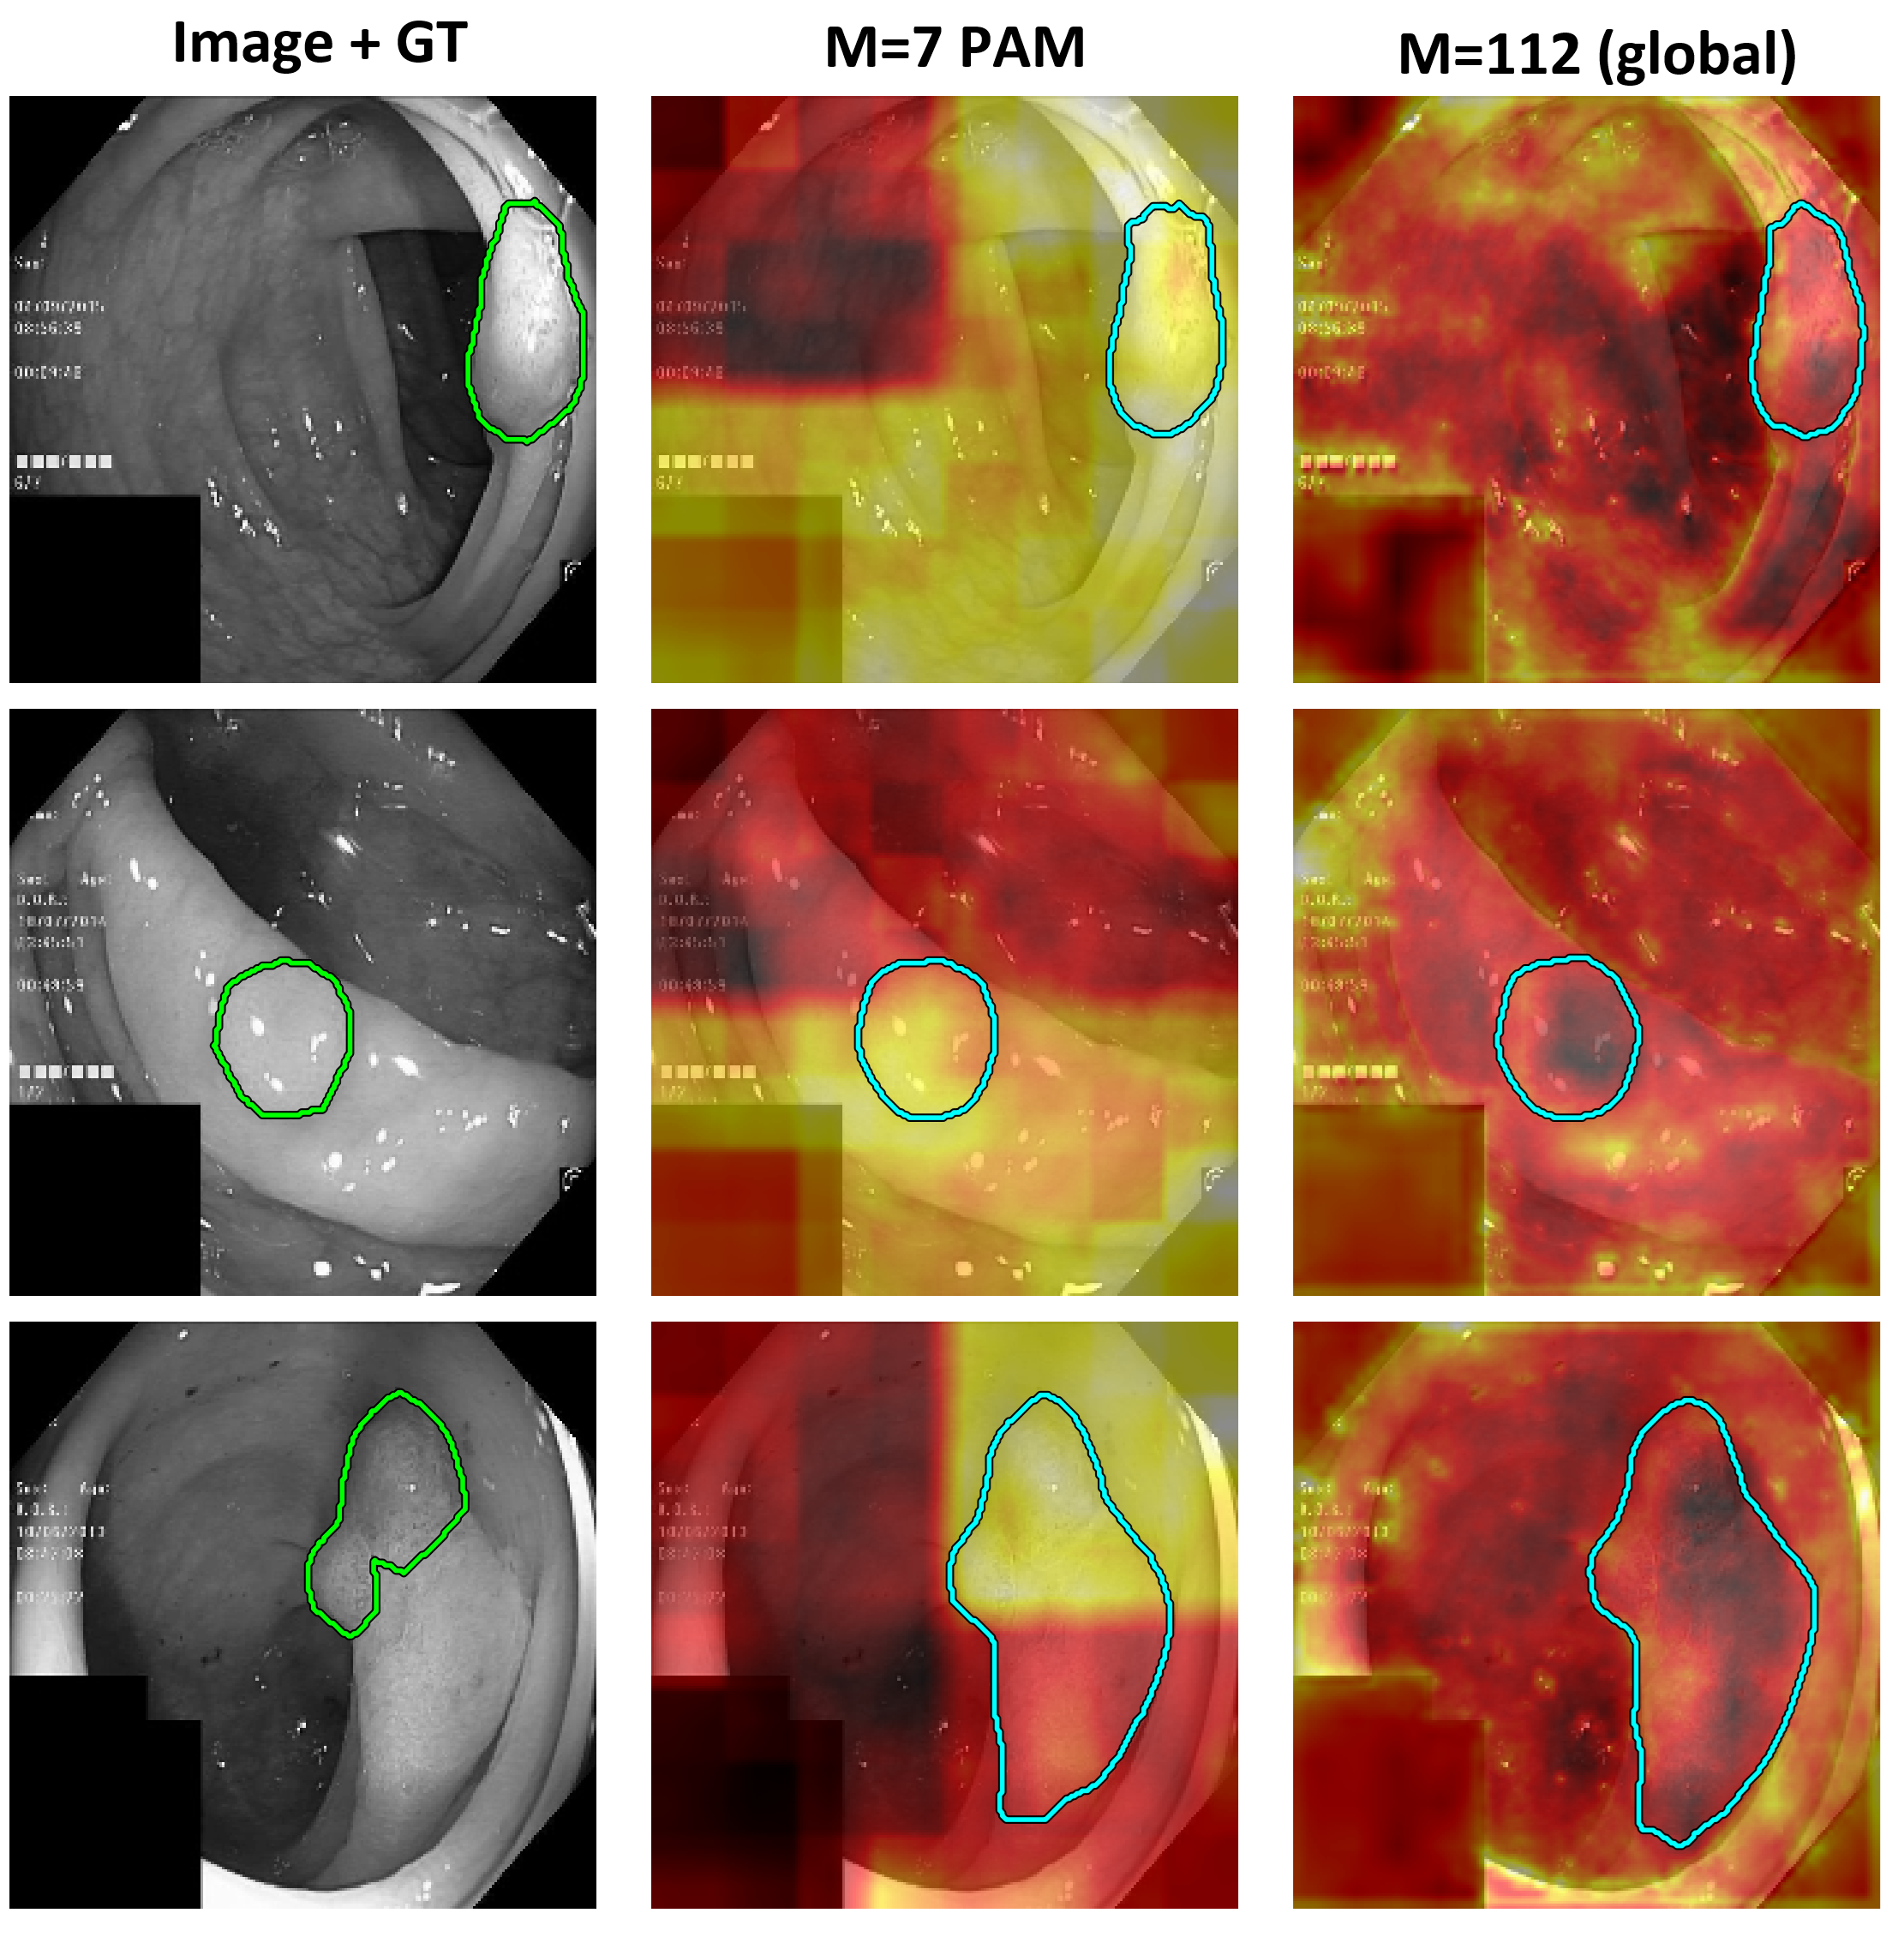
\includegraphics[width=\columnwidth]{figures/attn_Kvasir_M7_r32_pam_vs_M112.png}\\[-4pt]
  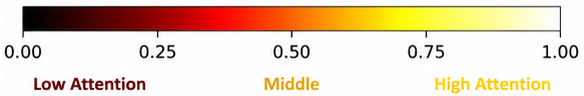
\includegraphics[width=0.68\columnwidth]{figures/hot_color_code.png}
  \caption{PAM contribution maps ($\|\text{output}-\text{input}\|_2$) on three Kvasir-SEG images. Each row: input with ground-truth contour (left), windowed PAM with $M{=}7$ (center), global PAM with $M{=}112$ (right). Each panel is normalized independently, so magnitudes are not comparable across panels.}
  \label{fig:attn_map}
\end{figure}

\subsection{Rank, Grouping, and Routing}
\label{sec:factors}

\begin{table}[t]
  \caption{Single-Factor Ablations on Synapse. Each block varies one factor; the others are fixed as indicated.}
  \label{tab:factors}
  \centering
  \footnotesize
  \setlength{\tabcolsep}{4pt}
  \begin{tabular}{@{}llcc@{}}
    \toprule
    Factor (fixed) & Setting & DSC$\uparrow$ & HD95$\downarrow$ \\
    \midrule
    \multirow{4}{*}{\shortstack[l]{Rank $r$\\($M{=}112$, PAM)}} & $r{=}16$ & \tbd{--} & \tbd{--} \\
                                   & $r{=}32$ & \tbd{79.44} & \tbd{27.26} \\
                                   & $r{=}64$ & \tbd{78.93} & \tbd{31.21} \\
                                   & no projection & \tbd{--} & \tbd{--} \\
    \midrule
    \shortstack[l]{Window only\\($M{=}28$, PAM)} & no projection & \tbd{--} & \tbd{--} \\
    \midrule
    \multirow{3}{*}{\shortstack[l]{Groups $G$\\(CAM-only)}} & $G{=}1$ & \tbd{--} & \tbd{--} \\
                                   & $G{=}4$ & \tbd{--} & \tbd{--} \\
                                   & $G{=}8$ & \tbd{78.26} & \tbd{30.59} \\
    \midrule
    \multirow{4}{*}{\shortstack[l]{Routing\\($M{=}7$, $r{=}32$)}} & PAM-only & \tbd{78.64} & \tbd{31.09} \\
                                   & CAM-only & \tbd{78.26} & \tbd{30.59} \\
                                   & fixed $g{=}0.5$ & \tbd{--} & \tbd{--} \\
                                   & learned & \tbd{77.78} & \tbd{34.29} \\
    \bottomrule
  \end{tabular}
\end{table}

Table~\ref{tab:factors} varies the remaining factors one at a time. Raising $r$ from 32 to 64 does \tbd{not} improve DSC, so in the tested range the window scale matters more than the rank. The no-projection rows use exact attention: at $M{=}112$ this is exact global PAM, which isolates the effect of the approximation from that of the routing, and at $M{=}28$ it removes the projection at the best Synapse window. $G$ is ablated under CAM-only routing, since the CAM branch does not contribute under PAM-only routing. \todo{grouping result.}

Among the routing modes, PAM-only routing performs best. The learned gate converged close to $g{=}0.5$ in our Synapse experiments and did not outperform PAM-only routing; we report this as an empirical observation and use PAM-only routing in the other experiments. \todo{optional: per-channel gate distribution / trajectory of the learned gate.}

\subsection{Limitations}
\label{sec:limitations}

Because Synapse and Kvasir-SEG have no validation split, their configurations were selected from the test-set ablations above, so the reported ApproxDA-TransUNet results on these datasets may be optimistic. The bias is bounded by the window-sensitivity range: small on Kvasir-SEG (\tbd{0.64} points), but up to \tbd{2.30} points on Synapse, where fine window selection is precisely what our results call for; in practice, $M$ should be tuned on held-out data. The study covers three datasets and a single backbone, and whether window sensitivity can be predicted without window ablations remains open.
